%% AMS-LaTeX Created with the Wolfram Language : www.wolfram.com

\documentclass[12pt]{article}
\usepackage{ceai} % Style file is in the project root.
\graphicspath{{../figs/}}

\begin{document}
\doublespacing	


\title{CE 488/5588: Applied Machine Learning\\ \large Topic 5: Introduction to Neural Networks}
\author{}
\date{}
\maketitle

In this topic, we will learn another supervised model---the artificial neural network (ANN). The idea behind ANNs is one of the most profoundly meaningful machine learning methodologies in modern artificial intelligence. The first ANN---called the \textit{perceptron}---was invented in the late 1950s by Frank Rosenblatt, a psychologist at Cornell University. Since then, ANNs, as an essential branch of AI, have experienced both highs and lows. Thanks to advances in deep neural networks (DNNs) and the breakthrough of convolutional neural networks (CNNs) by Geoffrey Hinton and his students (2012), ANNs (including various versions of DNNs and CNNs) have re-ignited AI, leading to transformative developments and applications.

\noindent\textbf{Learning objectives.} After completing this topic, you should be able to:
\begin{itemize}
    \item Write a single-neuron (perceptron) model in vector form and interpret the roles of weights and bias.
    \item Explain how common activation functions affect optimization (e.g., saturation/vanishing gradients, ``dying'' ReLUs).
    \item Choose appropriate output-layer/activation and loss pairs for binary classification, multi-class classification, and regression.
    \item Explain why a single linear decision boundary cannot solve XOR, and why hidden layers resolve this limitation.
    \item Describe (at a high level) how backpropagation applies the chain rule to compute gradients efficiently.
\end{itemize}

\vspace{0.5em}
\noindent\textbf{Terminology (to avoid common confusion).}
\begin{itemize}
    \item \textbf{Perceptron (classic):} a linear classifier with a hard threshold activation (step/sign) and the perceptron learning rule.
    \item \textbf{Logistic regression (single neuron):} a linear model with a sigmoid output interpreted probabilistically, typically trained with cross-entropy.
    \item \textbf{MLP:} a feedforward network with one or more hidden layers, trained via gradient-based methods/backpropagation.
\end{itemize}

\section{Neuron Cell and Perceptron}
\begin{figure}[ht]
    \centering
    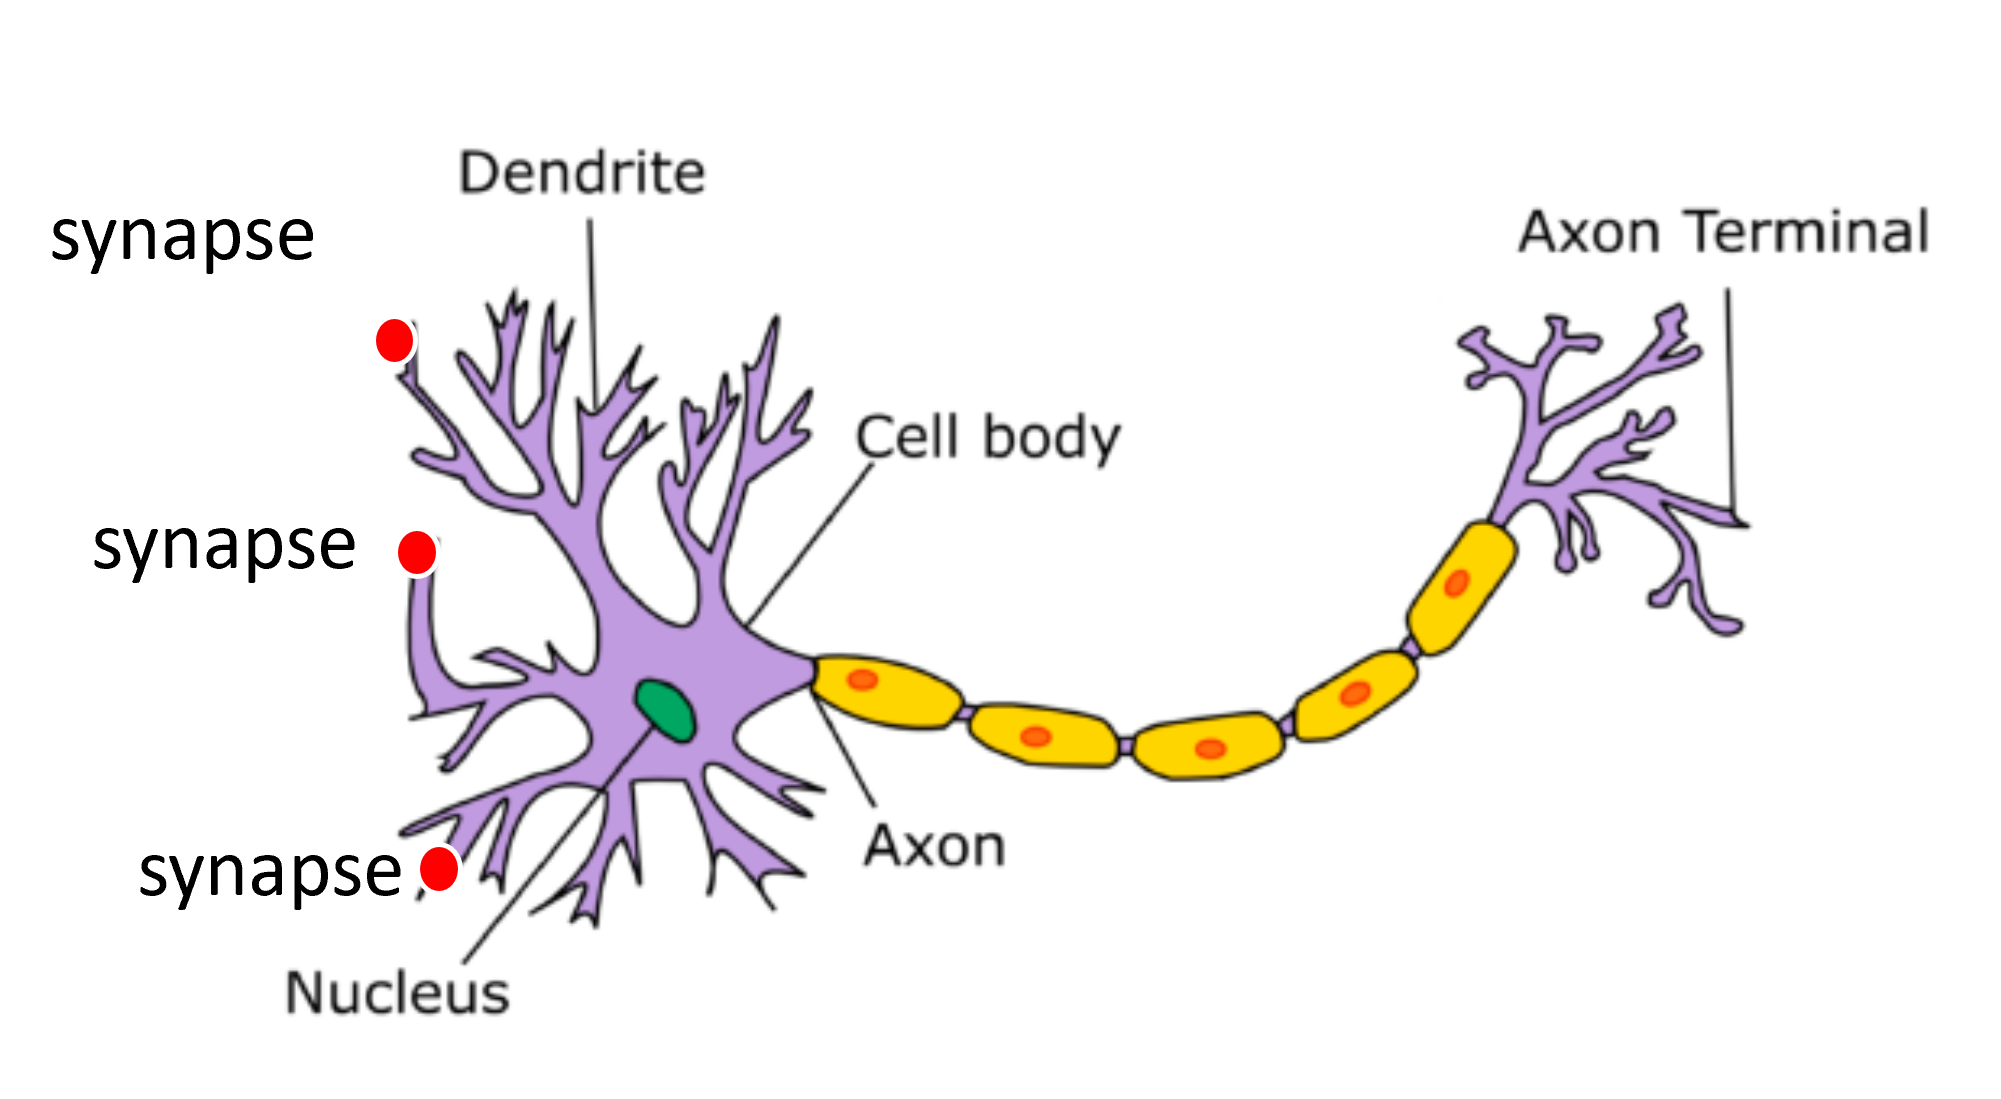
\includegraphics[width=0.75\textwidth]{Topic05fig01.png}
    \caption{Anatomy of a neural cell.}
    \label{topic05fig01}
\end{figure}
Neural activities in any life form are very complex, and a complete understanding remains elusive. Nonetheless, ANN computing is inspired by biological neural networks. As early as the 1940s and 1950s, pioneering researchers (Warren McCulloch and Walter Pitts) in psychology, biology, and mathematical logic proposed that the basic neural structure and mechanism could be simulated in a machine. Frank Rosenblatt built the first perceptron machine in 1958\footnote{You may search for images of it---it is a machine.}. As shown in Fig.~\ref{topic05fig01}, a neuron cell with its structural elements is illustrated, and some of their important functions are described below:
\begin{itemize}
    \item \textbf{Synapse:} the interface between neurons, which modifies or weights a signal from a nearby neuron.
    \item \textbf{Dendrites:} structures that bring signals to the cell body.
    \item \textbf{Cell body:} aggregates the input signals and activates the aggregated signal through a transformation.
    \item \textbf{Axons:} carry the activated signal from the cell body through the axon terminal to the next neuron.
\end{itemize}

By understanding a neuron cell in this way, we can represent its mechanism through mathematical modeling. Specifically, we consider that $D$ values are transmitted to the synapse, denoted by 
\[
    \bm{x} = [x_1, x_2, \cdots, x_D].
\]
After passing through the synapses, a weight is applied so that the signal becomes $w_i \cdot x_i$. The cell body aggregates these weighted signals (possibly adding an extra term), which is written as 
\[
    u(\bm{x}) = \sum_{i = 1}^{D} w_i \cdot x_i + b.
\]
Effectively, $u(\bm{x})$ defines a linear hyperplane function with intercept $b$. This linear summation is then transformed nonlinearly by an activation function $f(\cdot)$, which is written as 
\begin{equation}
\begin{split}
    y & = f[u(\bm{x})] \\
      & = f\Bigl(\sum_{i = 1}^{D} w_i \cdot x_i + b\Bigr)\\
      & = f\Bigl(\langle \bm{w}, \bm{x}\rangle + b\Bigr).
\end{split}
\label{t05eq01}
\end{equation}
The resulting value is then transmitted as a response signal, $y$, to the next neuron via the axon. A graph illustrating this mathematical model is shown in Fig.~\ref{t05fig02}. By comparing Fig.~\ref{t05fig02} with the anatomy of a neural cell in Fig.~\ref{topic05fig01}, one can see that the neuron model in Eq.~\ref{t05eq01} topologically simulates the mechanism of a neural cell. The model is called a perceptron---the simplest artificial neural network model. Unlike the original perceptron developed in 1958, the term “perceptron” now refers to an ANN unit, which is a building block of multi-layer ANNs.

\begin{figure}[ht]
\centering
\begin{subfigure}[b]{0.5\textwidth}
    \centering
    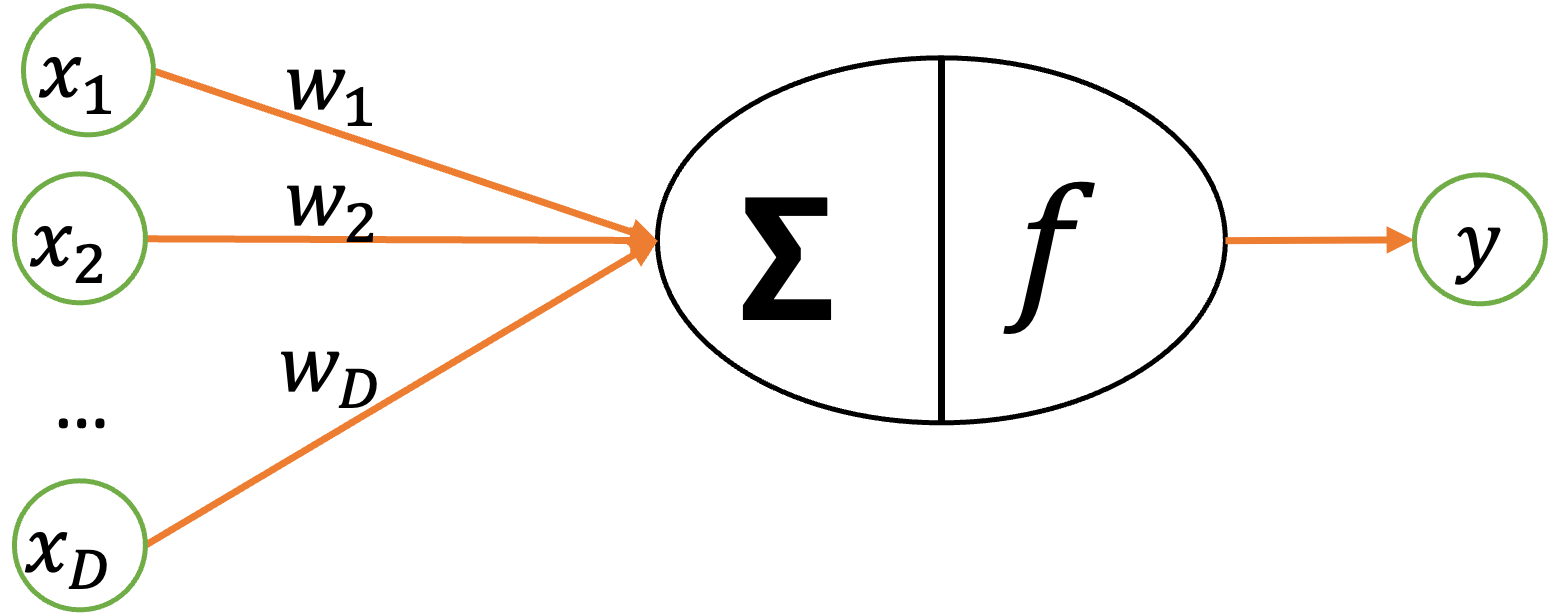
\includegraphics[width=1\textwidth]{Topic05fig02.png}
    \caption{}
    \label{t05fig02}
\end{subfigure}
\begin{subfigure}[b]{0.5\textwidth}
    \centering
    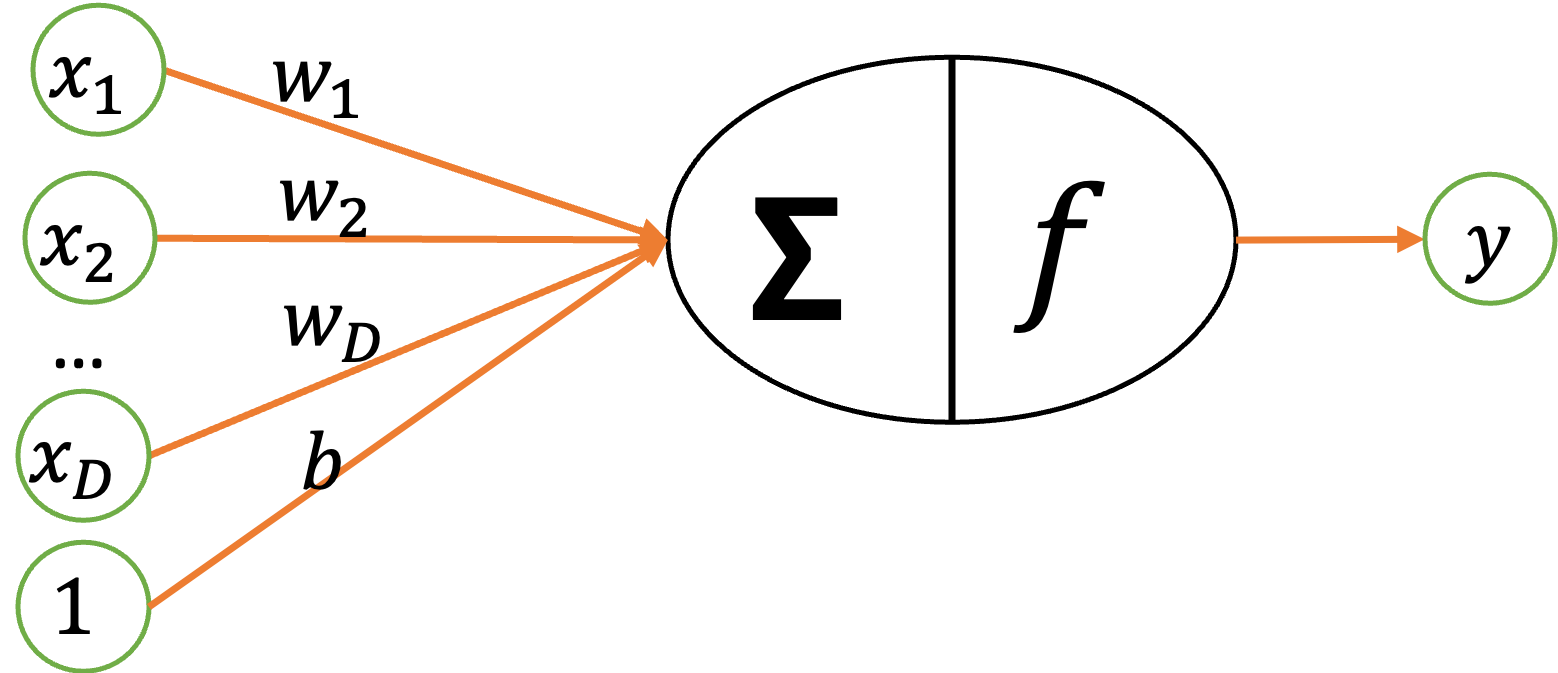
\includegraphics[width=1\textwidth]{Topic05fig03.png}
    \caption{}
    \label{t05fig03}
\end{subfigure}
\caption{Modeling a single neuron: (a) with an intercept in the neuron body; and (b) treating the neuron intercept as a weight by considering a unit input.}
\end{figure}

Note that one may treat the intercept $b$ in Eq.~\ref{t05eq01} as a weight parameter; in this way, an additional unit input can be appended to the input feature vector $\bm{x}$ (see Fig.~\ref{t05fig03}). Doing so, we obtain a more compact perceptron model:
\begin{equation}
\begin{split}
    y & = f[u(\bm{x})] \\
      & = f\Bigl(\sum_{i = 1}^{D} w_i \cdot x_i + b \cdot 1\Bigr)\\
      & = f\Bigl(\langle \bm{w}', \bm{x}'\rangle\Bigr),
\end{split}
\label{t05eq02}
\end{equation}
where \(\bm{w}' = [w_1, w_2, \cdots, w_D, b]\) and \(\bm{x}' = [x_1, x_2, \cdots, x_D, 1]\). In the following, we will simply write the perceptron model as \(f(\langle \bm{w}, \bm{x}\rangle)\) or \(f\left(\sum_i w_i x_i\right)\) without loss of generality.

\section{Perceptron as a Classifier}
\subsection{Activation}
Mathematically, the inner product or weighted summation creates a linear relation, \(u(\bm{x})\), between the weights (the model parameters) and the input feature vector \(\bm{x}\) in a perceptron. The activation function \(f(\cdot)\) then transforms this linear result into a response value \(y\).

The most common task for a perceptron is classification. In the binary classification case, the activation function can take one of two forms. One is the Heaviside step function:
\begin{equation}
    f_h(u)= \begin{cases} 
      1 & \text{if } u \geq 0, \\
      0 & \text{if } u < 0,
      \end{cases}
      \label{t05eq03}
\end{equation}
and the other is the sign function:
\begin{equation}
    f_s(u)= \begin{cases} 
      1 & \text{if } u \geq 0, \\
      -1 & \text{if } u < 0.
      \end{cases}
      \label{t05eq04}
\end{equation}

With a perceptron parameterized by a weight vector \(\bm{w}\), once \(\bm{w}\) is known the equation \(u(\bm{x}) = 0\) defines a decision boundary that separates the data points into two classes (either 0 and 1 or 1 and -1). In either case, the response \(y\) is a binary value based on thresholding \(u\).

An activation function that directly produces a classification label is called a \textit{hard-activation} function. Note that the sign function and the Heaviside function are essentially equivalent since \(2\,f_h(u)-1=f_s(u)\). However, hard-activation functions are not differentiable. An alternative is to use the standard logistic (sigmoid) function:
\[
    f(u) = \frac{1}{1+\exp(-u)},
\]
which is continuous and differentiable; such activations are called \textit{soft-activation} functions.

There are many activation functions in practice; Table~\ref{tab01} lists some commonly used ones.
\begin{table}[ht]
\centering
\begin{tabular}{|l|l|p{6cm}|}
\hline
\textbf{Activation Function} & \textbf{Equation} & \textbf{Description} \\
\hline
Sigmoid & \(f(u) = \frac{1}{1 + e^{-u}}\) & Maps input to a range between 0 and 1, useful for binary classification. \\
\hline
Hyperbolic Tangent (tanh) & \(f(u) = \tanh(u)\) & Maps input to a range between -1 and 1; often preferred for hidden layers. \\
\hline
Rectified Linear Unit (ReLU) & \(f(u) = \max(0, u)\) & Allows only positive values, mitigating the vanishing gradient problem. \\
\hline
Leaky ReLU & \(f(u) = \max(\alpha u, u)\) & Allows a small gradient when the input is negative to avoid dying neurons. \\
\hline
Exponential Linear Unit (ELU) & \(f(u) = \begin{cases} 
u & \text{if } u > 0, \\
\alpha(e^u - 1) & \text{if } u \leq 0,
\end{cases}\) & Smooths the negative side, helping the cost converge faster. \\
\hline
\end{tabular}
\caption{Commonly Used Activation Functions in Neural Networks.}
\label{tab01}
\end{table}

Besides the sigmoid and tanh functions, one activation function worth mentioning is the Rectified Linear Unit (ReLU), defined as
\begin{equation}
 \mathrm{ReLU}(u) = \max(0, u) = 
\begin{cases}
    u, & \text{if } u \geq 0,\\[1ex]
    0, & \text{if } u < 0.
\end{cases}
\end{equation}
ReLU is widely used in modern deep neural networks due to its computational simplicity.

\subsection{Perceptron Learning}
Estimating the model parameters (contained in \(\bm{w}\)) from data is a core task in machine learning. As we have learned from logistic regression, we first construct a loss function and then minimize it to estimate the model parameters. Consider the training data
\[
\mathcal{D} = \{ (\bm{x}_i, y_i) \mid i = 1, 2, \cdots, N\},
\]
where \(x_i \in \mathbb{R}^D\) and \(y_i \in \{-1, 1\}\).

We consider two types of activation functions:
\begin{itemize}
    \item \textbf{Hard-activation functions} (\(f_H\)), using either the Heaviside or sign function.
    \item \textbf{Soft-activation functions} (\(f_S\)), such as the sigmoid, which is bounded between 0 and 1. (Through appropriate scaling, the tanh function, bounded between -1 and 1, can be obtained via \(\tanh(u)=2\,\mathrm{Sigmoid}(u)-1\).)
\end{itemize}

When using the hard-activation sign function, the loss for the \(i^\text{th}\) training example can be defined as
\begin{equation}
\begin{split}
        l_i & = |y_i - y_i^*|\\[1ex]
            & = \bigl| f_H\bigl(\langle \bm{w}, \bm{x}_i\rangle\bigr) - y_i^* \bigr|.
\end{split}
\label{t05eq05}
\end{equation}
The loss takes on two possible values: 0 when the prediction is correct and 2 when it is wrong:
\begin{itemize}
    \item If \(y_i = 1\) and \(y_i^* = 1\), or \(y_i = -1\) and \(y_i^* = -1\), then \(l_i=0\).
    \item If \(y_i = 1\) and \(y_i^* = -1\), or \(y_i = -1\) and \(y_i^* = 1\), then \(l_i=2\).
\end{itemize}
This can be extended to the general situation when using the soft-activation functions where the activated values as predictions are continuous.
\begin{equation}
\begin{split}
        l_i & = |y_i - y_i^*|\\[1ex]
            & = \bigl| f\bigl(\langle \bm{w}, \bm{x}_i\rangle\bigr) - y_i^* \bigr|.
\end{split}
\label{t05eq06}
\end{equation}


The total loss is then expressed as the sum of the individual losses:
\[
L(\bm{w}) = \sum_{i = 1}^{N} \bigl| f\bigl(\langle \bm{w}, \bm{x}_i\rangle\bigr) - y_i^* \bigr|.
\]

Thus, estimating the model parameter vector \(\bm{w}\) becomes an optimization problem:
\begin{equation}
    \bm{w}^* = \mathrm{argmin}_{\bm{w}}\, L(\bm{w}).
    \label{t05eq08}
\end{equation}

While logistic regression yields a convex optimization problem, the optimization for a perceptron is not necessarily convex.\footnote{In the presentation above, we effectively used an $L_1$ (absolute-difference) loss to measure prediction error. In modern neural networks (e.g., MLPs), it is common to use an $L_2$ loss (squared error), i.e., to square the absolute difference, which yields a smooth objective that is convenient for gradient-based optimization.}

\subsection{Solution to the Perceptron}
The perceptron’s goal is to find a separating hyperplane if one exists. The algorithm iteratively adjusts the weights based on misclassified examples without explicitly calculating the gradient over the entire dataset. Note that the loss surface as a function of \(\bm{w}\) is non-convex.

The good news is that if the training data \(\mathcal{D}\) is \textit{separable} and a hard-activation function is used, then a global solution always exists (i.e., the iterative process converges, as has been classically proven). The bad news is that many global loss-minimizing solutions exist—in this case, for separable data, the minimum loss is zero for all solutions. Such a simple perceptron with hard-activation has been classically described as a logical-gate operator; in fact, a perceptron can realize logical operators such as `AND', `OR', and `NOR'. Fig.~\ref{t05fig04a} illustrates the 'AND' gate.
% \begin{figure}[ht]
% \centering
% \begin{subfigure}[b]{0.45\textwidth}
%     \centering
%     \includegraphics[width=1\textwidth]
% Topic05fig04a.png
%     \caption{}
%     \label{t05fig04a}
% \end{subfigure}
% \begin{subfigure}[b]{0.45\textwidth}
%     \centering
%     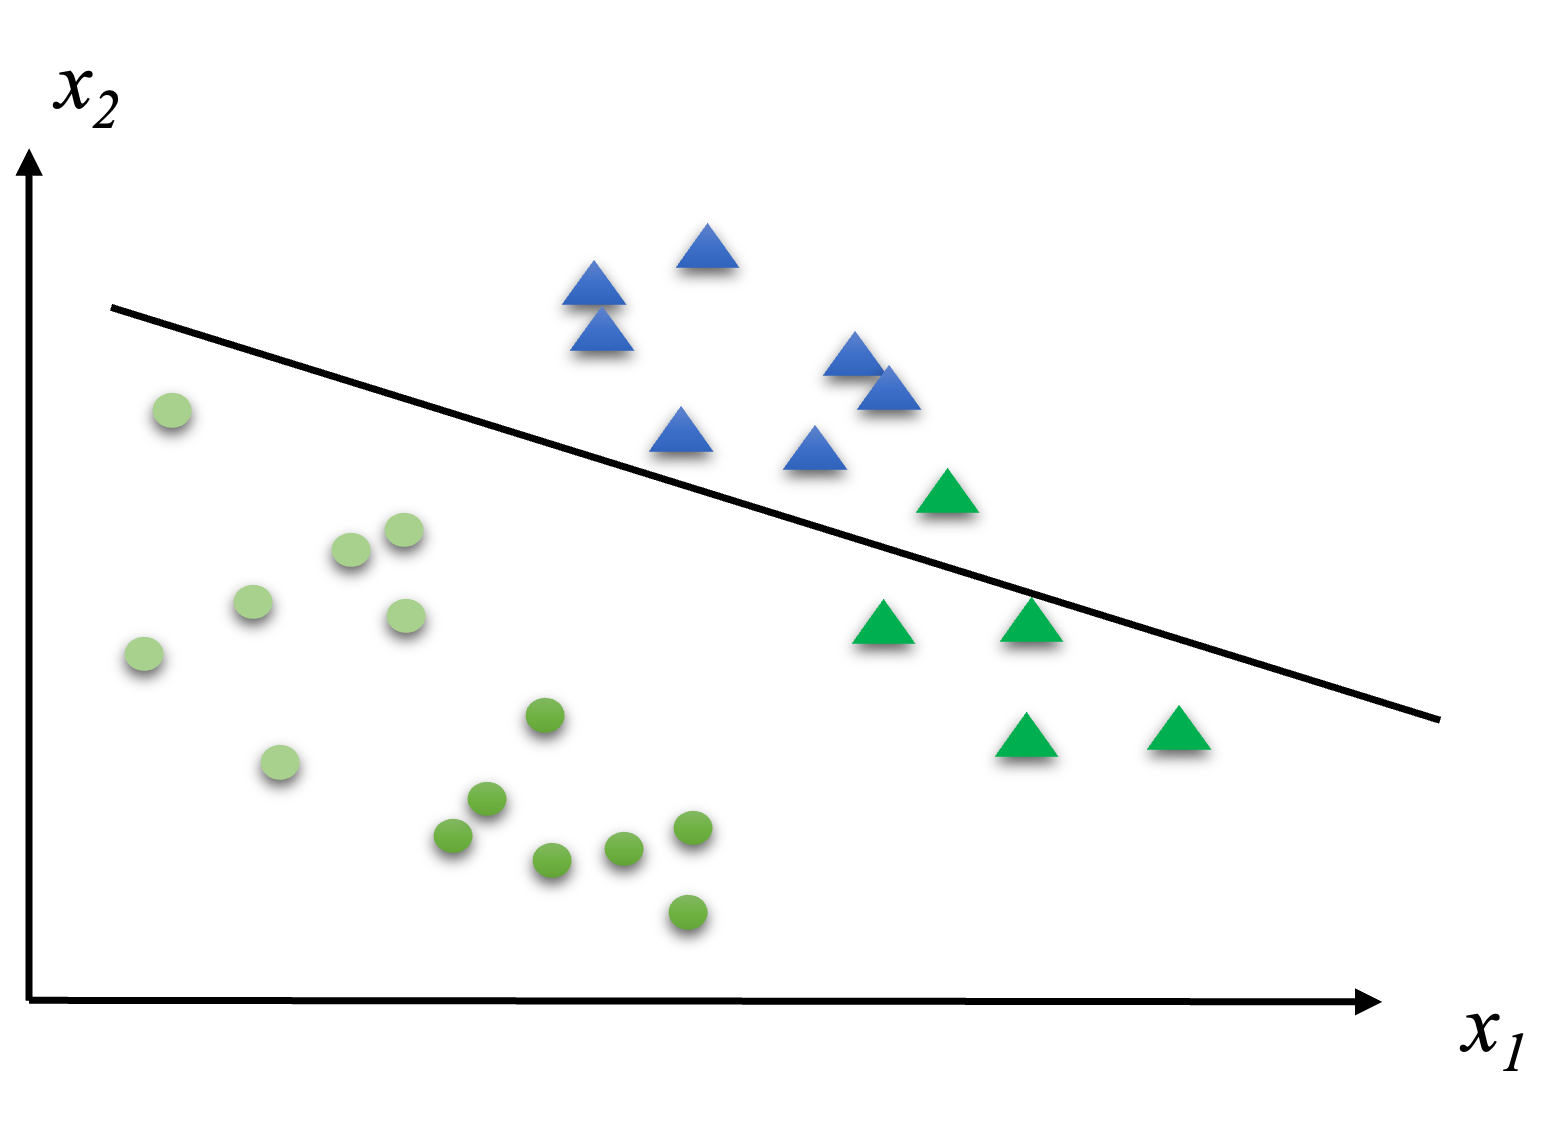
\includegraphics[width=1\textwidth]{Topic05fig04b.png}
%     \caption{}
%     \label{t05fig04b}
% \end{subfigure}
% \caption{Decision boundary for (a) separable data points and (b) non-separable data points. For non-separable data, a nonlinear decision boundary is necessary.}
% \end{figure}

\begin{figure}[ht]
\centering
\begin{subfigure}[b]{0.45\textwidth}
  \centering
  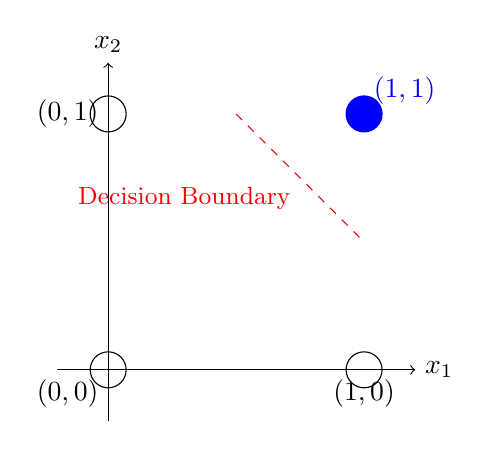
\begin{tikzpicture}[scale=3.25]
   % Draw axes
    \draw[->] (-0.2,0) -- (1.2,0) node[right]{$x_1$};
    \draw[->] (0,-0.2) -- (0,1.2) node[above]{$x_2$};
    
    % Plot negative points (open circles)
    \draw (0,0) circle (2pt) node[below left] {$(0,0)$};
    \draw (0,1) circle (2pt) node[left] {$(0,1)$};
    \draw (1,0) circle (2pt) node[below] {$(1,0)$};
    
    % Plot positive point (filled blue circle)
    \filldraw[blue] (1,1) circle (2pt) node[above right] {$(1,1)$};
    
    % Draw decision boundary for the AND gate (e.g., x1 + x2 = 1.5)
    % The line passes through (0.5,1) and (1,0.5)
    \draw[dashed, red] (0.5,1) -- (1,0.5) node[midway, below left] {\small Decision Boundary};

  \end{tikzpicture}
  \caption{Linearly separable configuration (forming an AND gate).}
  \label{t05fig04a}
\end{subfigure}
\hfill
\begin{subfigure}[b]{0.45\textwidth}
  \centering
  \begin{tikzpicture}[scale=1.25]
    % Draw axes
    \draw[->] (-0.5,0) -- (3,0) node[right]{$x_1$};
    \draw[->] (0,-0.5) -- (0,3) node[above]{$x_2$};
    
    % Plot positive examples (filled blue circles)
    \filldraw[blue] (0.5,0.5) circle (3pt) node[below left] {+$\,$};
    \filldraw[blue] (2.5,2.5) circle (3pt) node[above right] {+$\,$};
    
    % Plot negative examples (open circles)
    \draw (0.5,2.5) circle (3pt) node[above left] {$-\,$};
    \draw (2.5,0.5) circle (3pt) node[below right] {$-\,$};
  \end{tikzpicture}
  \caption{Non-separable (XOR) configuration.}
  \label{t05fig04b}
\end{subfigure}
\caption{Examples of data configurations in \(x_1\)-\(x_2\) space.}
\label{t05fig04}
\end{figure}


If a soft-activation function is used, the non-uniqueness is removed because the loss function becomes convex, as in logistic regression.

The fundamental weakness of a perceptron (and logistic regression) is that its decision function, \(u(\bm{x}) = \langle \bm{w}, \bm{x}\rangle\), is linear. Therefore, if the data are not separable, zero loss cannot be achieved. Although a perfect model may not be realistic for complex data, striving for a perfect model is an initial objective\footnote{When taking a model-centric approach, the goal is to design a high-performance ML model with the highest possible accuracy.}.

Fig.~\ref{t05fig04b} shows a case where the four data points for a non-separable case; in case, a linear decision function \(u(\bm{x})=0\) leads to nonzero loss.

To enhance the capacity of a perceptron, one stacks multiple perceptrons to form a network. The resulting model is called a multi-layer perceptron (MLP).

\section{Multi-layer Perceptron}
\subsection{Architecture}
An MLP is a form of artificial neural network (ANN) known as a feedforward neural network (FF-NN). FF-NNs are characterized by a network of neurons arranged as a directed acyclic graph, where data is transmitted from the input layer to the output layer and full connections are not necessary. An MLP is a specific type of fully connected FF-NN that has one or more hidden layers between the input and output layers. Each neuron in a hidden layer receives input from the previous layer and passes its output to the next layer. More specific FF-NN's exist, such as the radial-basis ANN\footnote{A radial-basis neural network (RB-NN) has three layers, including one hidden layer, and uses a radial basis function as its activation function.}. By extending an MLP, one can construct an ANN with tens to hundreds of layers, known as a deep neural network (DNN). Recent advances in AI have largely focused on DNNs.

The architecture of an MLP is illustrated in Fig.~\ref{t05fig05}.
\begin{figure}[ht]
    \centering
    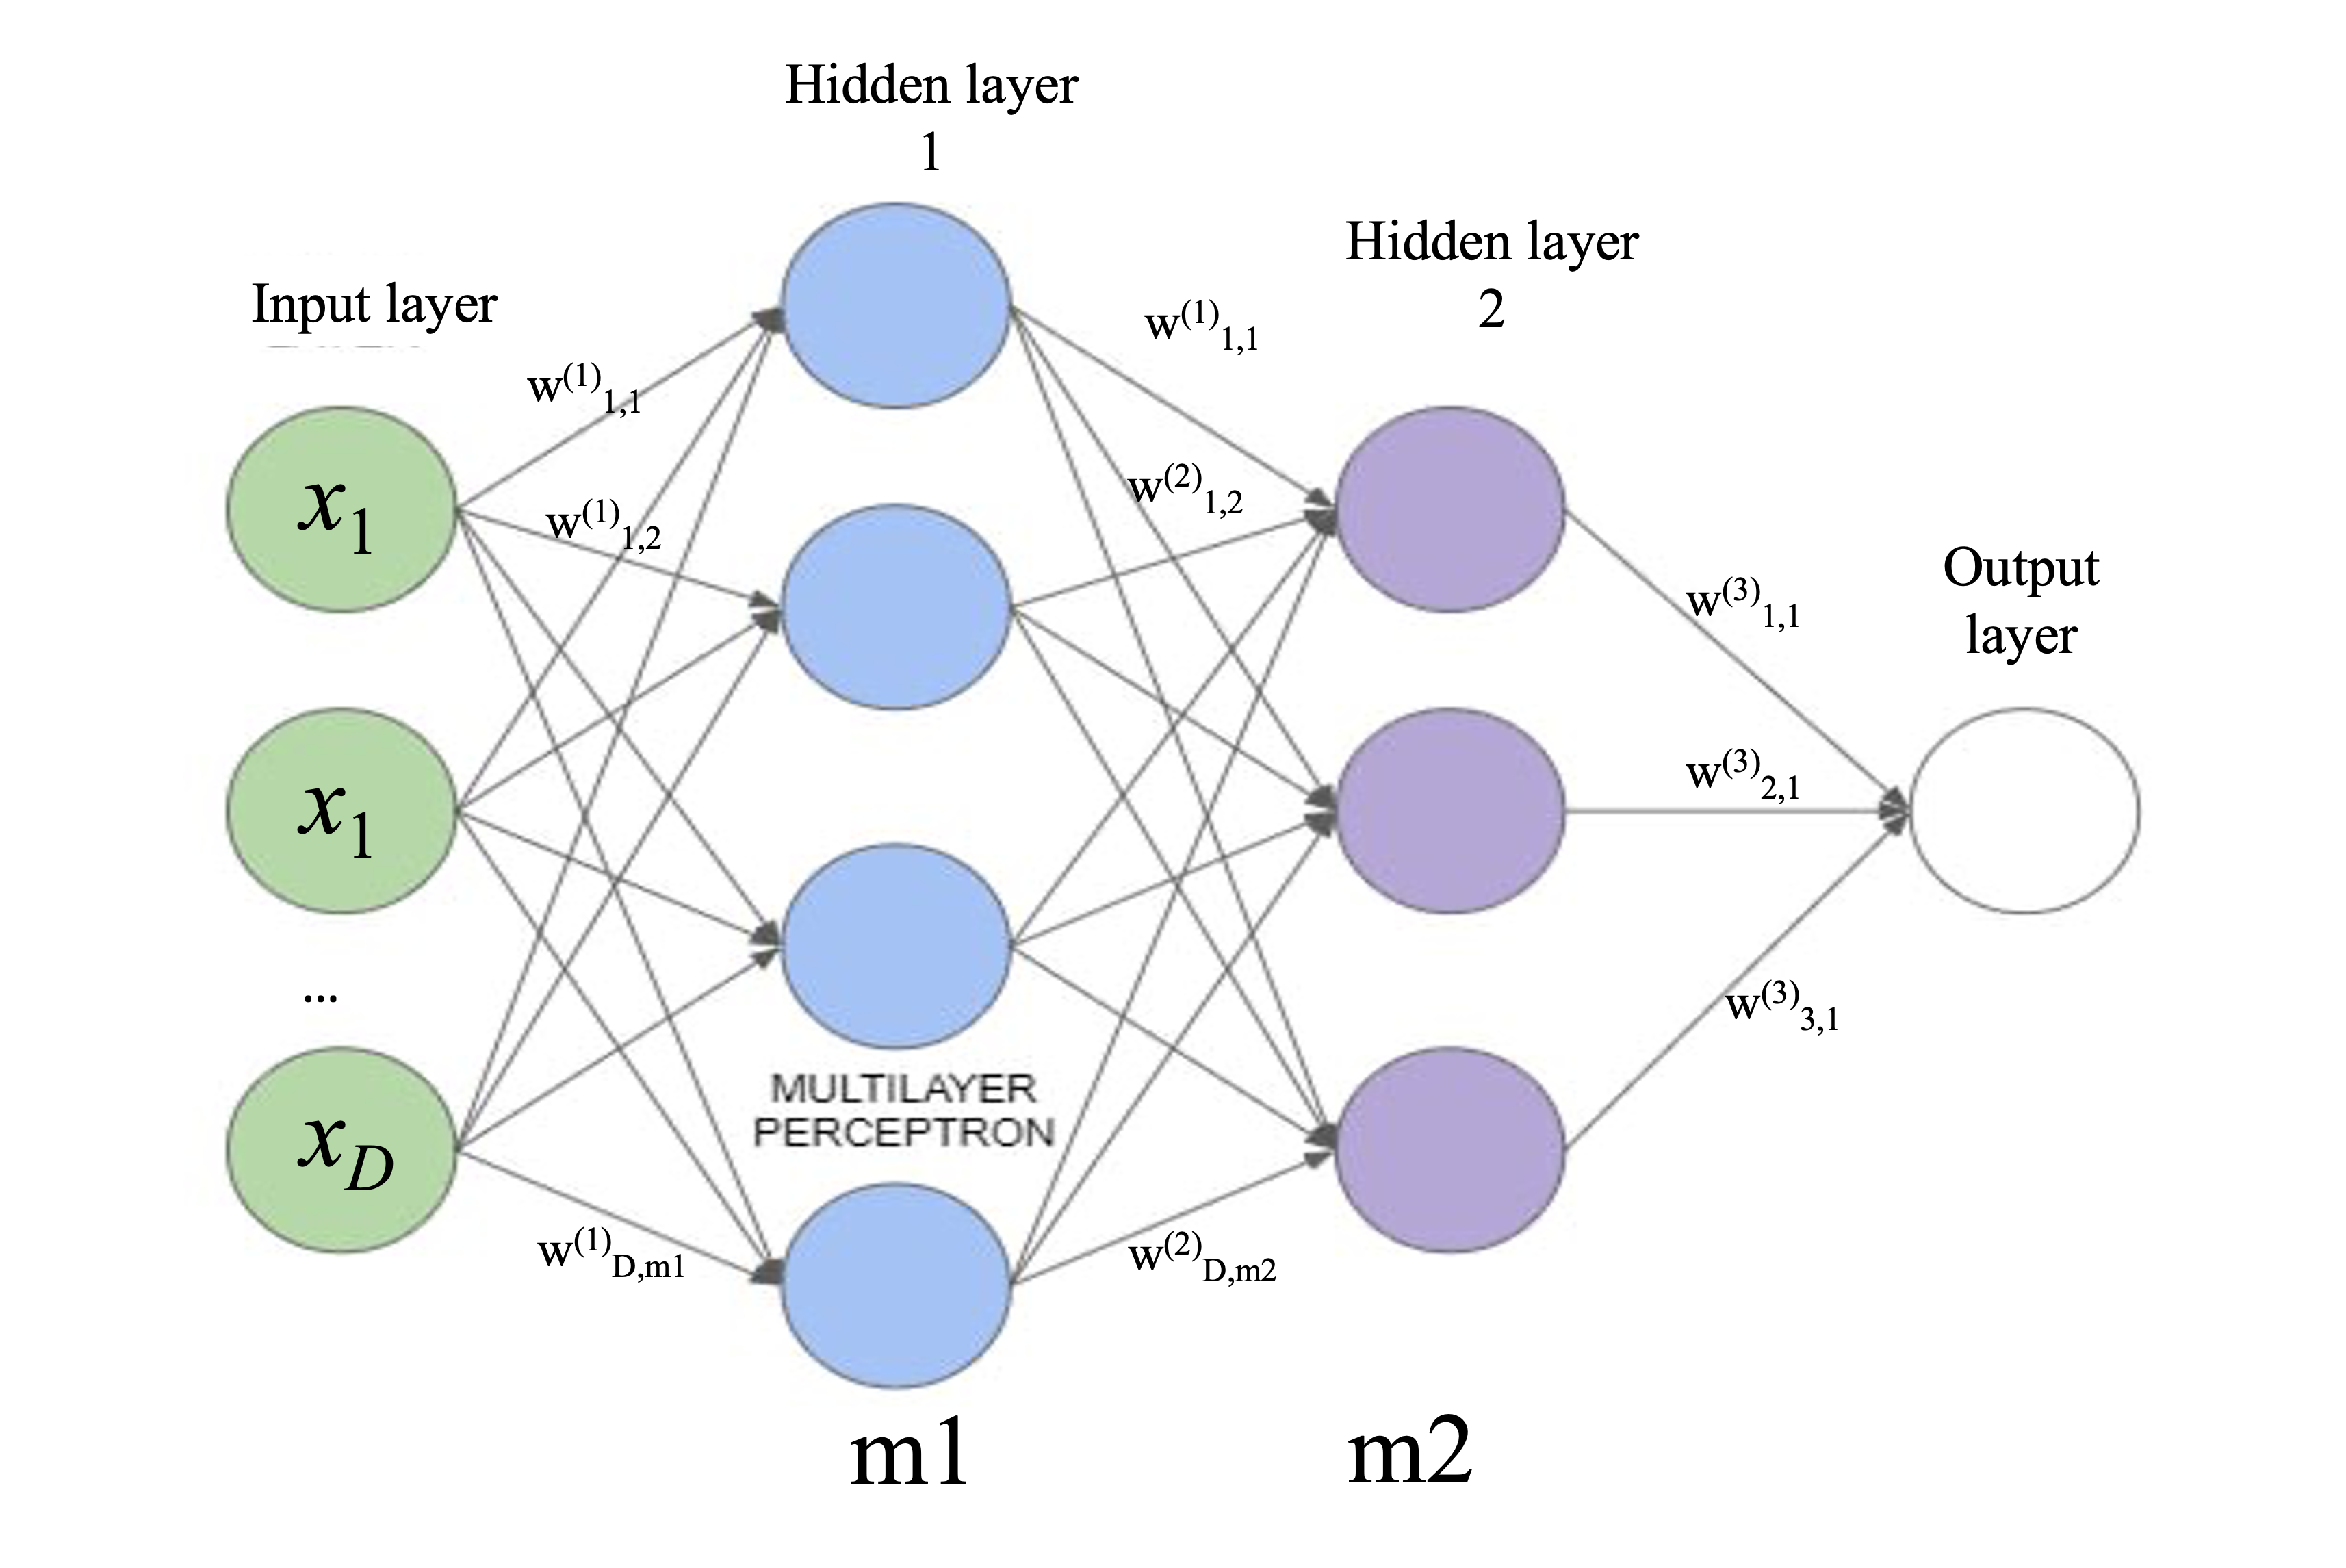
\includegraphics[width=1\textwidth]
    {Topic05fig05.png}
    \caption{Decision boundary for (a) separable data points and (b) non-separable data points. For non-separable data, a nonlinear decision boundary is necessary.}
    \label{t05fig05}
\end{figure}
The key feature of an MLP is the introduction of one or more hidden layers that are \textit{fully connected} with both the preceding and subsequent layers. Within each hidden layer, several neurons perform two operations: aggregation via a weighted summation (i.e., an inner product) and activation through a nonlinear function.

Suppose the input feature \(\bm{x}\) is a \(D\)-dimensional vector (e.g., \(D=3\)); let the first hidden layer have \(m_1\) neurons (say, \(m_1=4\)), the second hidden layer have \(m_2\) neurons (e.g., \(m_2=3\)), and the output layer (for binary classification) consist of one neuron. With full connectivity, the weighting configuration can be described as:
\begin{itemize}
    \item \textbf{Input to the 1st hidden layer:} a weight \(w_{j,k}^{(1)}\) defines the connection from the \(x_j\) feature to the \(k^\text{th}\) neuron.
    \item \textbf{1st hidden layer to 2nd hidden layer:} a weight \(w_{j,k}^{(2)}\) defines the connection from the \(j^\text{th}\) neuron of the 1st hidden layer to the \(k^\text{th}\) neuron of the 2nd hidden layer.
    \item \textbf{2nd hidden layer to the output layer:} a weight \(w_{j,1}^{(3)}\) defines the connection from the \(j^\text{th}\) neuron of the 2nd hidden layer to the output neuron.
\end{itemize}
In general, we denote the weight connecting the \((l-1)^\text{th}\) layer to the \(l^\text{th}\) layer as \(w_{j,k}^{(l)}\). Furthermore, at the \(l^\text{th}\) layer (excluding the input layer), an activation function \(f^{(l)}(\cdot)\) is applied. For the three-layer MLP in Fig.~\ref{t05fig05}, using a compact inner-product notation, the operation between the \((l-1)^\text{th}\) and \(l^\text{th}\) layers is repeated \(m_l\) times, and the aggregation can be represented as a matrix-vector product. Define
\[
    \bm{W}^{(l)} = \{w_{j,k}^{(l)}\}.
\]
The aggregation from the \((l-1)^\text{th}\) layer to the \(l^\text{th}\) layer is then
\[
    \bm{W}^{(l)} \bm{x} \quad \text{(if the \((l-1)^\text{th}\) layer is the input layer)}
\]
or
\[
    \bm{W}^{(l)} \bm{f}^{(l-1)} \quad \text{(if the \((l-1)^\text{th}\) layer is a hidden layer)}.
\]

Thus, for a three-layer MLP, the output can be written as:
\begin{equation}
    y = f^{(3)}\Bigl( {\bm{W}^{(3)}}^T f^{(2)}\bigl( {\bm{W}^{(2)}}^T f^{(1)}\bigl( {\bm{W}^{(1)}}^T \bm{x} \bigr) \bigr) \Bigr).
\end{equation}
This represents a nested chain of matrix-vector products and activation operations. Note that the activations \(f^{(1)}\) and \(f^{(2)}\) are vector-valued. Examining the chain of operations, we see that after the first inner-product operations at different neurons, the activation at the first hidden layer transforms the result nonlinearly. The output of that hidden layer becomes the new input for the next hidden layer. Consequently, the decision function cannot explicitly defined as in a perceptron (as $u(\bm{x}) = <\bm{w}, \bm{x}> = 0$); at the space of $\mathbb{R}^D$ for the input $\bm{x}$, the resulting decision `plane' will be highly nonlinear. 


\subsection{MLP Learning}
Learning an MLP is not trivial because the model is highly nonlinear. Although the basic idea is to minimize a total loss function, the numerical procedure is much more complex than for a single perceptron.

The most commonly used algorithm is back-propagation. Its essence is straightforward. If the total loss function is defined as\footnote{Here, the absolute prediction error is squared. For multi-class classification, the output of $y$ is vector-valued, so it is more convenient to define the loss as the squared norm of the error vector.}
\begin{equation}
L = \sum_i \left|  f^{(3)}\Bigl( {\bm{W}^{(3)}}^T f^{(2)}\bigl( {\bm{W}^{(2)}}^T f^{(1)}\bigl( {\bm{W}^{(1)}}^T \bm{x} \bigr) \bigr) \Bigr) - y_i^* \right|^2,
\label{t05eq09}
\end{equation}
and if we denote the prediction vector and true label vector as \(\bm{y}\) and \(\bm{y}^*\) respectively, then the loss can be written compactly as
\[
    L = \|\bm{y} - \bm{y}^*\|^2.
\]
In gradient descent procedures to minimize \(L\), the gradient with respect to each weight matrix \(\bm{W}^{(l)}\) is determined using the chain rule, propagating the error backward from the final layer to the first hidden layer. This is why the algorithm is called backpropagation. (Many excellent online resources cover these details; see, e.g., \href{http://neuralnetworksanddeeplearning.com/chap2.html}{this resource}.)

Some general observations:
\begin{itemize}
    \item In general, the loss function surface is non-convex.
    \item Common gradient descent methods do not guarantee a global solution---they may converge to a local minimum or a saddle point (e.g., Gauss-Newton gradient descent).
\end{itemize}

To date, stochastic gradient descent (SGD) methods have proven most effective for training neural networks, with many variants such as AdaGrad and Adam being widely adopted. For large-scale deep neural networks with high-dimensional inputs (e.g., images), selecting an appropriate SGD method is crucial.

Moreover, with the recent strides in generative AI, the technical challenges of training vast network models have largely been addressed, shifting the focus to empirical strategies for training. This includes careful selection of methods, precise tuning of the learning rate, and the strategic use of regularization techniques.
\begin{itemize}

    \item Learning Rate: The learning rate dictates the step size in weight updates during training. An optimal learning rate is essential: too high and the model might diverge; too low and convergence becomes painfully slow. Adaptive methods like AdaGrad and Adam, along with scheduling strategies (e.g., learning rate decay), offer mechanisms to automatically fine-tune the learning process.

    \item Regularization: Regularization methods such as weight decay (L2), L1 regularization, dropout, and early stopping are integral to preventing \textit{overfitting}. They ensure that the model not only fits the training data but also generalizes well to unseen data. These techniques are especially critical when training MLPs or feedforward networks, where over-parameterization is a common risk.
\end{itemize}

We will encounter these settings during our numerical practice and homework of developing MLP models. 

\section{Beyond MLP}
In the realm of ANNs, there are many different types of neural networks. The MLP is the most basic model for understanding ANNs, characterized by its feedforward and fully connected architecture. If the fully connected constraint is relaxed, a more general ANN called a feedforward neural network can be formed.

\subsection{Feedforward Neural Network}
A feedforward neural network is a general term for any neural network in which connections between units do not form a cycle. This category includes MLPs as a specific instance but also encompasses other architectures that do not necessarily follow a strictly layered, fully connected structure. The key features include:
\begin{itemize}
    \item Information flows in only one direction---from input nodes, through any hidden nodes, to output nodes; there are no cycles or loops.
    \item Feedforward neural networks can have various structures, such as different connectivity patterns or types of neurons and activation functions.
\end{itemize}

\subsection{ANN Overview in a Table}
Many other types of ANNs exist in modern AI literature. The classic ones include recurrent neural networks, long short-term memory (LSTM) networks, and self-organizing maps (SOMs). In recent years, deep neural networks such as convolutional neural networks (CNNs) and generative adversarial networks (GANs) have gained prominence. The following table provides an overview of these ANNs.

\newgeometry{margin=1cm} % Modify this if you need even more space
\begin{landscape}
\begin{table}[ht]
\centering
\begin{tabular}{|p{3cm}|p{8cm}|p{5cm}|p{5cm}|}
\hline
\textbf{Type of ANN} & \textbf{Definition} & \textbf{Key Characteristics} & \textbf{Typical Applications} \\
\hline
Multi-Layer Perceptron (MLP) & A feedforward neural network with one or more hidden layers between its input and output layers, using nonlinear activation functions. & Fully connected layers; backpropagation training. & Classification; regression. \\
\hline
Convolutional Neural Network (CNN) & A deep learning algorithm for processing data with a grid-like topology, such as images. & Convolutional layers; pooling layers; fully connected layers. & Image recognition; video analysis; image classification. \\
\hline
Recurrent Neural Network (RNN) & A network where connections between nodes form a directed graph along a temporal sequence, enabling dynamic temporal behavior. & Sequential data processing; feedback loops. & Time series analysis; natural language processing; speech recognition. \\
\hline
Long Short-Term Memory (LSTM) & A special kind of RNN capable of learning long-term dependencies, designed to mitigate the long-term dependency problem. & Gating mechanisms; sequence prediction. & Sequence prediction; time series forecasting; text generation. \\
\hline
Generative Adversarial Network (GAN) & A framework consisting of two neural networks contesting with each other, designed to generate new data with the same statistics as the training set. & Generator and discriminator networks; zero-sum game dynamic. & Image generation; art creation; photorealistic images. \\
\hline
Autoencoder & A network used to learn efficient representations (codings) of data, typically for dimensionality reduction or feature learning. & Encoder and decoder; feature learning. & Data compression; feature extraction; image denoising. \\
\hline
Radial Basis Function (RBF) Network & A type of feedforward neural network that uses radial basis functions as activation functions, typically used for function approximation, classification, and regression. & Radial basis function in the hidden layer; function approximation. & Function approximation; classification; system control. \\
\hline
Feedforward Neural Network (FNN) & A broad category of neural networks in which connections between units do not form cycles, including MLPs, CNNs, and RBF networks. & Unidirectional flow of data; no cycles or loops. & Pattern recognition; classification; regression analysis. \\
\hline
\end{tabular}
\caption{Overview of Popular Artificial Neural Networks.}
\label{table:ANNs}
\end{table}
\end{landscape}


\newgeometry{margin=1in} 
\doublespacing	

\section{Conclusion}
In this topic, we explored the fundamental building blocks of artificial neural networks, starting with the perceptron model and its biological inspirations. We examined various activation functions and loss models, and discussed the limitations of single-layer perceptrons for complex, non-separable data. The transition to multi-layer perceptrons (MLPs) was shown as a natural extension to enhance model capacity through additional hidden layers and nonlinear transformations, leading to the powerful deep neural networks used in modern AI. This foundation sets the stage for further exploration of advanced neural architectures and training algorithms in subsequent topics.

\end{document}
